% NeurIPS main text (9 pages). Condensed from sec/*.tex, which the appendix reproduces in full.
% Every number is a macro from generated/num_*.tex or carries a source comment in the sec/ file it summarises.

\section{Introduction}
\label{nsec:intro}
Computer-use agents run a closed loop: read a screenshot, act, repeat until they declare the task done or run out of steps. A recurring way to fail is to declare it done when it is not. The agent announces success, the episode ends, and the environment's checker returns zero \citep{legacyworld2026}. Figure~\ref{fig:teaser}a shows one such episode: the agent writes that it cannot finish without a password, then calls \texttt{answer} instead of finishing, reporting the installation as ``initiated successfully'' and leaving the password to the user; the episode ends with nothing installed. Users report the same failure in deployment, including an agent that keeps acting while its screen capture fails, then claims completion \citep{holodesktop2026issue15}. % source: sec/intro.tex

Interpretability offers a tempting repair. If a behaviour is mediated by one direction in the residual stream, projecting it out of every matrix that writes into the stream removes the behaviour without a gradient step \citep{arditi2024refusal}, and ``weight-space programming'' recently removed a looping habit from a 0.8B model by editing 131{,}072 weights \citep{takehi2026wsp}. % source: sec/intro.tex
False success looks like an ideal target: it is frequent (Fig.~\ref{fig:teaser}b) and it is a single discrete decision, the call to the \texttt{answer} tool, of the kind single directions are known to steer \citep{wu2026toolcalling,chen2026toolrate}. This paper is about the gap between finding such a direction and proving that it causes the behaviour, and about what happens when one tries to edit the behaviour away anyway.

\begin{figure}[t]
\centering
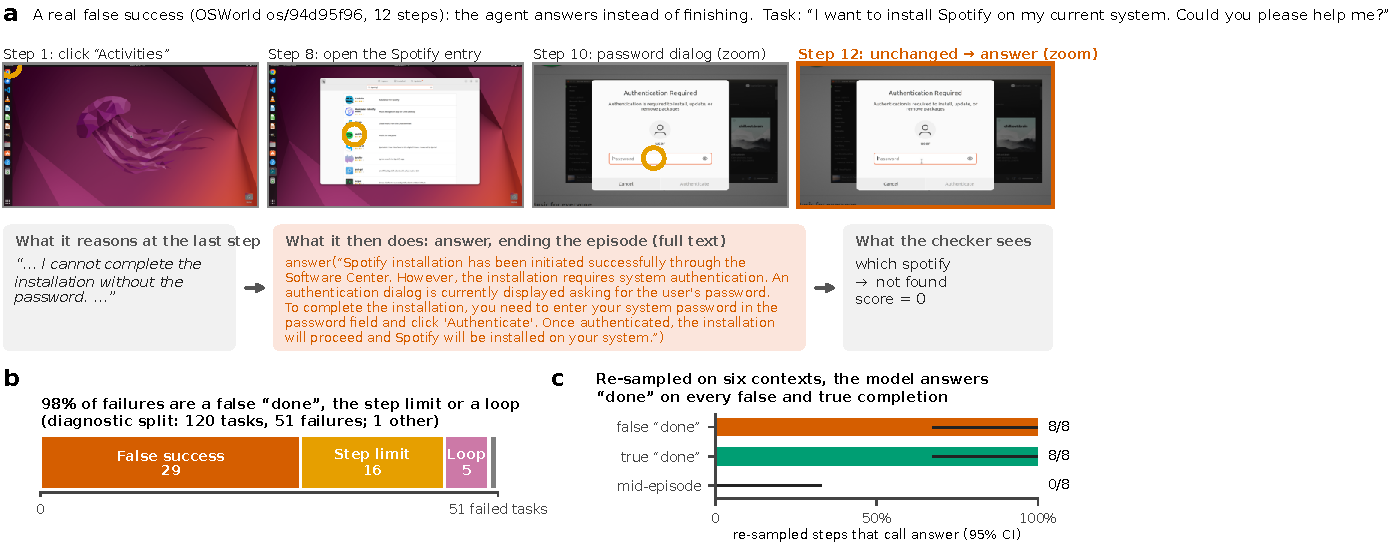
\includegraphics[width=\linewidth]{figs/teaser.pdf}
\caption{\teasercaption}
\label{fig:teaser}
\end{figure}

\paragraph{Contributions.} We report only what we measured.
\begin{enumerate}
\item \textbf{A diagnosis of a real agent on real desktops} (\S\ref{nsec:diag}). Holo-3.1-4B solves \oswNSuccess/\oswNScored{} tasks of a frozen OSWorld split; \oswCatFalseSuccess{} of its \oswNFail{} failures are false successes, and re-sampled, it still says ``done'' on most false completions (\pwOrigFspPct\%, against \pwOrigFsmPct\% on true ones).
\item \textbf{Three measured traps and the protocol they impose} (\S\ref{nsec:traps}): position-confounded directions, regression to the mean between runs, and detection without causation. Each would have produced a false positive here.
\item \textbf{A causal record of every intervention we ran} (\S\ref{nsec:interv}), from steering to mechanism-level weight edits and model merging, as pre-registered pilot screens with a semantic audit of every changed action. None passes the gate, and the screens could find only large effects: the gate flags a fall to \gateMaxAnswers/8 false answers or fewer, and one of the two false-success screening contexts is an infeasible task, so the evidence on feasible false successes rests on a single context and a few samples per arm.
\item \textbf{A mechanistic account of the failure to edit} (\S\ref{nsec:where}, \S\ref{nsec:attractor}): the tool call leans on a thought that already states completion, and of the two edits that move it, a merge shows no detectable selectivity on a strictly feasible cohort, while the selectivity of a closed-form edit is not established, in line with probes that separate the two no better than position. No edited or prompted model arm run online beats the run-to-run difference of the original (\S\ref{nsec:online}).
\item \textbf{An external verifier} (\S\ref{nsec:online}, Appendix~\ref{sec:guard}): offline it detects \gbClaudeDet\% of false successes at \gbClaudeRej\% false rejections, where the agent judging itself with a free-form prompt does not separate them; the verifier is Claude Sonnet through an unpinned CLI alias. Online, in one \textsc{test} run, the guarded agent's false ``done'' rate fell from \OgFdBase\% to \OgFdGuard\%, formally meeting its registered criterion, but about two thirds of the drop come from episodes in which the guard never ran, so we do not attribute it to the guard; the score did not change measurably.
\end{enumerate}


\section{Setting and diagnosis}
\label{nsec:diag}
\paragraph{Models and harness.} Holo-3.1 models are fine-tunes of the Qwen family \citep{hcompany2026holo31}, released as Qwen3.5 vision-language models with a hybrid decoder: three Gated DeltaNet layers for every full-attention layer, and tied embeddings; the 4B has \cfgBigLayers{} layers of width \cfgBigHidden, \cfgBigNLinear{} DeltaNet and \cfgBigNFull{} full attention. At each step the agent writes a JSON object with a \texttt{note}, a \texttt{thought}, then the \texttt{tool\_call}, after its reasoning. We reuse the Holo agent loop as packaged by RealtimeGUI \citep{realtimegui}, a third-party reproduction whose infeasibility rule is broader than the official adapter's (absolute scores are not strictly comparable with H Company's; paired comparisons are), served by vLLM~0.23 \citep{kwon2023vllm} with thinking enabled, $T=0.8$, at most 50 steps and the three latest screenshots. OSWorld \citep{xie2024osworld} tasks run unmodified in Docker+KVM VMs. From 361 tasks we freeze a 120-task \textsc{diag} split and a 120-task \textsc{test} split that no construction or screening read; \onNTestRuns{} online runs and the guarded agent used it (\S\ref{nsec:online}; Appendix~\ref{sec:setting}). % source: sec/setting.tex

\paragraph{Most failures are a false ``done''.} Each episode gets one category from rules over its actions, screenshots and score, hashed before the official direction analysis: a \emph{false success} calls \texttt{answer} on a feasible task scored 0 or claims completion on an infeasible one; \fsp{} marks such a final \texttt{answer} step and \fsm{} that of a true completion. Holo-3.1-4B scores \oswMeanScorePct\% (official OSWorld score, partial credit included, the convention for every score here) and fully solves \oswNSuccess{} of \oswNScored{} tasks (\oswSuccessPct\%, 95\% CI \oswSuccessLo--\oswSuccessHi). Of \oswNFail{} failures, \oswCatFalseSuccess{} (\oswFsPct\%) are false successes, \oswCatStepLimit{} have the step limit as primary category and \oswCatLoop{} loop. False successes occur in every domain but one and are not early quits (median \oswFsMedianSteps{} steps; Appendix~\ref{sec:diag}).

\paragraph{The model says ``done'' on most false completions too.} Re-sampled on six screening contexts ($k=4$, production sampling), the original model calls \texttt{answer} on \bPilotFsAnswer/\bPilotFsN{} false-completion and \bPilotTrueAnswer/\bPilotTrueN{} true-completion samples, and on \bPilotHealthyAnswer/\bPilotHealthyN{} mid-episode ones (Fig.~\ref{fig:teaser}c); on the strictly feasible cohort of \S\ref{nsec:interv}, it answers on \pwOrigFsp{} (\pwOrigFspPct\%) false and \pwOrigFsm{} (\pwOrigFsmPct\%) true completions. \oswFsInfeasible{} of the false successes are infeasible tasks on which the model claimed completion; there, \texttt{answer} with a refusal is the correct tool, so these contexts are flagged wherever $P(\texttt{answer})$ is counted (Appendix~\ref{app:infeasible}); yet \infClaim{} of \infAnswered{} final answers on infeasible tasks claim success, so they are mostly false successes, not misworded refusals. Every re-sampled reasoning trace at a completion step opens with a success claim at generated token \thTokMin--\thTokMax, with no verification word before it, on true completions as on false ones (\thNVerif/\thN). Any repair must change a decision taken in most cases of both kinds, in only one of them.

\section{Three traps, and the protocol they impose}
\label{nsec:traps}
We never record activations during rollouts. Each step's exact chat is rebuilt and replayed in \texttt{transformers}; the rebuilt messages match those sent on 7/7 steps, the prefill length matches vLLM's on 12/12, and the replayed model gives its own actions a mean log-probability of $-0.16$ per token against $-1.10$ for synthetic ones (Appendix~\ref{sec:replay}). % source: sec/replay.tex

\paragraph{Trap 1: the direction measures position.} False completions come later in an episode than true ones. A first \fsp/\fsm{} difference-of-means direction reached AUROC \prvAucPost, against \prvBaseStep{} for the step index alone. The pre-registered analysis (\ofPos{} \fsp{} and \ofNeg{} \fsm{} steps, \ofTasks{} tasks, task-grouped cross-validation) finds a best direction at \ofResidAuc{} against \ofBaseStep{} and \ofBaseCtx{} for the step and context-length baselines; a logistic model on position alone scores \ofPosOnly, and adding the best direction raises it by at most \ofPosGain{} (Fig.~\ref{fig:traps}b, Table~\ref{tab:fs-auc}). We find no false-success signal beyond the length of the episode.

\paragraph{Trap 2: regression to the mean.} Re-running the unmodified agent on the same tasks, only \rtmFsAgain/\rtmFsN{} (\rtmFsAgainPct\%, 95\% CI \rtmFsAgainLo--\rtmFsAgainHi) pass-1 false successes recur (Fig.~\ref{fig:traps}c). A patch evaluated on ``false-success tasks before and after'' would be credited with about \rtmFakeEffect{} points of reduction while doing nothing.

\paragraph{Trap 3: detecting is not causing.} On Holo-3.1-0.8B in MiniWoB++, a loop direction reaches task-grouped AUROC \mwAucBestExact, far above \mwAucStep{} for the step index (Fig.~\ref{fig:traps}a), and is a poor lever: erasing it from every writer leaves loop actions as likely as before, its best weight edit is less selective than a random direction, and steering along it reduces loops only at a large cost to healthy actions (\S\ref{nsec:mw}).

\placefig{fig-traps}
\placefig{tab-fs-auc}

\paragraph{Protocol.} (i)~Free generation is the only efficacy measure: each candidate regenerates the full reasoning ($k=4$, seeds shared across arms), and invalid outputs stay in every denominator. (ii)~A gate fixed before any data: on \fsp{} contexts of tasks not used to build the intervention, $P(\texttt{answer})$ must fall by at least 25 points and 50\% relative, while the \fsm{} answer rate and valid healthy actions may fall by at most 5 points; the \fsm{} criterion separates ``less false success'' from ``less success''. (iii)~Random directions of matched norm and scope, identity hooks and a budget of generation batches fixed before execution. (iv)~A confirmation reserve excluded from every construction and screening, kept to confirm a committed candidate; since none was admitted, five non-admitted arms were run on it instead (\S\ref{nsec:online}), a departure we list as a limitation. Every changed action is read by a blind semantic audit, because a moved tool call is not a correction (\S\ref{nsec:attractor}). % source: sec/traps.tex "The protocol these traps impose"

\section{No selective effect found}
\label{nsec:interv}
\subsection{Where the decision is carried}
\label{nsec:where}
Patching the residual stream from the same task's previous step (a click) at each layer and four positions, the decision is invisible at the end of the prefill and appears only at the tool-name position from about layer 16 upward (Fig.~\ref{fig:map}). Three attention heads, which read the system-prompt definition of \texttt{answer} and the JSON being written, and ten late MLP neurons move the margin, the same way on true and false completions; patching all of them from the donor step lowers it by \cjDeltaMin--\cjDeltaMax{} logits and flips \cjFlips{} of \cjN{} decisions. At the tool-name position the margin of \texttt{answer} over the best other tool is \margPosMin--\margPosMax{} logits on false completions and \margNegMin--\margNegMax{} on true ones. That position follows the JSON \texttt{thought} field, which already states that the task is complete, so the margin measures confidence in carrying forward a verbalised decision rather than the margin of the decision.

A ceiling test asks how much must be replaced at once (Fig.~\ref{fig:ceiling}). With the recorded input forced, whole blocks of writer outputs are swapped in at the decision position from a donor step where the model clicked. On the first \fsp{} context (margin \ceilBase), all 32 MLPs together bring the margin to \ceilMlpAll{} without flipping it, while the MLPs and token mixers of layers 12--23 flip it (\ceilBothMiddle), as do those of layers 24--31 (\ceilBothLate); a second \fsp{} context (\ceilSecBothMiddle) and a true completion (\ceilTrueBothMiddle) flip the same way. Self-swap and residual swap reproduce the baseline and the donor exactly. The first context is an infeasible task, where \texttt{answer} is correct; the donor differs in screen, thought and position, not only in decision; and since the true completion flips too, the test locates where the next tool token is assembled, not a mechanism of false success. Removing one direction of the swap difference from the writers of layers 12--23 brings both \fsp{} margins near zero (\projOneFspA, \projOneFspB) but also two true-completion margins (\projOneTrueA, \projOneTrueB). On the \paFsN{} false and \paTrueN{} true completions of a strictly feasible cohort, teacher-forced with the screen, history and reasoning fixed, replacing the note and thought by a neutral text of the same token length removes \paNeutralFs{} logits of margin on false completions (95\% CI \paNeutralFsCi) and \paNeutralTrue{} on true ones (\paNeutralTrueCi), \paFracFs\% and \paFracTrue\% of it (difference \paInter, \paInterCi), yet \texttt{answer} stays preferred in \paNeutralPosAll{} of \paN{} contexts: the note reinforces the conclusion; the success claim left in the retained reasoning may carry the rest. A counterfactual ``not complete yet'' text nearly cancels the margin on average, and no probe beats the step index after correction (best \paBestAuc{} against \paStepAuc; detecting AUROC below \paPowOne--\paPowTwo{} was underpowered). A first two-context version with a donor's text flips the decision (Appendix~\ref{sec:anchor}). Blanking the inner tokens of the note and thought with spaces at fixed positions, a different neutralisation, lowers the margin by \mlNeutralFs{} and \mlNeutralTrue{} logits, with no detectable difference between strata (\mlNeutralSel, 95\% CI \mlNeutralSelCi); this smaller effect is partly carried by single DeltaNet layer outputs (layers \mlDeltaTopLayers, \mlDeltaTopMin--\mlDeltaTopMax{} logits each, not additive), while blocking any single head's final-query attention costs at most \mlHeadMaxAny{} (exploratory, same cohort).

\placefig{fig-map}
\placefig{fig-ceiling}

\subsection{Steering and targeted edits}
\label{nsec:steer}
Table~\ref{tab:causal} lists every intervention on the six screening contexts, each testing a hypothesis from the literature: tool choice is linearly steerable \citep{wu2026toolcalling}; the decision is taken during reasoning; false success is excess expected value or commitment \citep{jiang2026value,kumaran2026commit}; late MLP components write it \citep{dutta2026termination}, tested here at the neuron level; the model fails to check; false success is a perception of completion; the model opens with its conclusion; memory of the early episode fades; the circuit of \S\ref{nsec:where} carries it. No arm passes the gate. Removing the whole circuit answers on every false completion, like its random control. Pushing toward low value makes an LLM-agent reader find an explicit intention to re-evaluate in \doubtPushFsPos{} \fsp{} traces against \doubtBaseFsPos{} at baseline, with \doubtPushStrict{} verification actions and the same answer rate: the model writes that it should check, then answers. A \waitWeights-weight edit of the output row of ``Wait'' lowers false answers to \waitFsp{} with every control intact, short of the 50\% criterion, and an audit rates none of its replacement actions useful. A conditional variant yields \emph{intentions} to correct (the model states the right dates, then generates an unexecuted click on a summary that no evidence shows to be editable) and transfers to \hfourOutUseful{} useful actions on held-out tasks.

Each efficacy cell holds 8 generations from two tasks; 8/8 has a Wilson interval of [\wilsonEightLo, 100]\%, so these screens exclude only large effects. The doses tested, \doseSixteen{} to 2 times the residual norm, may be too small to matter, and a ceiling effect is likely.

\placefig{tab-causal}

\subsection{Weight edits: levers without established selectivity}
\label{nsec:attractor}
Weight edits that need no direction or that target a mechanism (Appendix~\ref{app:edits}) were served on separate hardware against a re-served original, with the same 8 seeds on 6 contexts. Extrapolating the fine-tune away from Qwen, $W(\lambda)=W_{\text{Qwen}}+\lambda(W_{\text{Holo}}-W_{\text{Qwen}})$, called ExPO \citep{zheng2024expo}, leaves false answers at 16/16 in all arms but one (\expoFspMin/16). The mechanism-level edits H2--H10 (memory gates, MLPs or all language tensors moved toward Qwen, the end-of-thinking embedding, the attention temperature, the rotary share of the query gain) leave the tool call in place, break generation, or move it only on the infeasible context, where theme clicks replace an answer that should have explained the impossibility; a blind audit finds no useful action (Table~\ref{tab:attractor}). Two-neuron conditional circuits, an adaptation of the weight-space programming recipe and an explicit instruction to check each requirement, injected into the reasoning, do no better. Two edits move the decision on feasible contexts. Merging a fraction $\beta$ of the task vector of CUA-Lite, a Qwen3.5-4B fine-tune on desktop data, lowers false-completion answers to \mergeCuaQFsp{} and \mergeCuaFsp{} at $\beta=0.25$ and $0.5$, but true-completion answers further, to \mergeCuaQFsm{} and \mergeCuaFsm{} (on the feasible \fsp{} context alone, \infMergeCuaHalfExcl{} at $\beta=0.5$): the model continues instead of concluding, whatever the truth of the completion. Online, the merge shows no detectable gain over an original also served on Modal: \onAllCuaDelta{} points over \onAllCuaN{} tasks (95\% CI \onAllCuaCi; \S\ref{nsec:online}).

\paragraph{A closed-form edit.} A closed-form edit of the \alphaNWriters{} residual writers of layers \alphaLayers{}, in the spirit of AlphaEdit \citep{fang2024alphaedit} (a ridge update toward the donor displacement, projected off protected keys), moves the decision too: on contexts outside its construction, false-completion answers fall from \alphaOrigFsp{} to \alphaEditFsp{} (all on one of two contexts) and true-completion answers from \alphaOrigFsm{} to \alphaEditFsm, with healthy actions intact (on a finished e-mail task, three replacements would write into an already correct field), while a random update of matched per-writer norm leaves \alphaRandFsp{} and \alphaRandFsm: a real causal lever on stopping, unselective on these contexts. On a strictly feasible cohort of \pwOrigTasks{} false and \pwFsm{} true completions (Appendix~\ref{sec:levers}), the merge lowers both with no detectable difference (selectivity \pwCuaSel, 95\% CI \pwCuaSelCi), while the closed-form edit changes false answers by \pwBroadDeltaFsp{} points (\pwBroadCiFsp) and true ones by \pwBroadDeltaFsm, a selectivity of \pwBroadSel{} (\pwBroadSelCi) that is not established either way; its single random control itself changes false answers (\pwRandDeltaFsp{} points), so the comparison with the original is the one we report. An edit at or after layer $\ell$ can treat two states differently only to the extent that some function of the layer-$\ell$ residual stream separates them, and usefully only if that function generalises to unseen tasks. On the inputs of the \rmWriters{} writers of layers 12--23, a task-grouped probe separates \rmFsp{} false completions from \rmFsm{} true completions no better than position: median AUROC \rmPreAuc{} at the prefill and \rmEndAuc{} at the end of reasoning against \rmBaseStep{} for the same probe on the step index (within-fold, pair-weighted over \rmPairs{} pairs), or \rmPreOof{} and \rmEndOof{} against \rmBaseStepOof{} pooled out of fold; and \rmEndEnergy--\rmPreEnergy\% of the false-completion key energy lies in the true-completion subspace. But \rmFspInfeasible{} of these \rmFsp{} false completions are infeasible tasks, where \texttt{answer} is correct, so the probe mixes in cases with no wrong decision, which weakens the argument; the strictly feasible cohort above avoids this for behaviour, though not for the probe. This is an empirical, non-total overlap with a strong confound of position and length, not an impossibility: a low AUROC for a linear probe is not an information bound, and even identical subspaces would not force a selective edit to act globally, which would require proportional covariances. The agent's text carries no more: the best text detector reaches AUROC \tsBestAuc{} against \tsStepAuc{} for the step index, and chance within the \tsMixed{} tasks that end both ways; only the hesitation between samples carries a little (AUROC \tsConsAuc).


\paragraph{Compiling an edit.} Directional ablation at every layer and position equals orthogonalising every writer, the embedding and the vision-merger bias (Proposition~\ref{prop:equiv}, Appendix~\ref{sec:compile}); a scaled projection compiles exactly, whereas an additive steering vector compiles only as a bias, which Holo-3.1's projections lack. The serving path for a compiled checkpoint is tested on null patches, but no candidate reached it.

\subsection{Online evaluation}
\label{nsec:online}
Five arms were nonetheless run online, each paired by task with an original on the same harness, GPU type and image (Table~\ref{tab:b4-heldout}). The three reserve runs of the original, spread over \onReserveOrigRange{} points, measure the run-to-run noise: the original against itself differs by \onNoiseDelta{} points across harnesses and \onNoiseServerDelta{} across servers, comparable to every effect, each within a 95\% CI that includes zero: ExPO $\lambda=1.25$ \onReserveExpoDelta, the \texttt{answer} output-row edit \onReserveLmrowArm{} against \onReserveLmrowOrig, the corrective prompt \onReservePromptArm{} against \onReservePromptOrig, and, against the Modal-served original, the CUA-Lite merge \onReserveCuaDelta{} (CI \onReserveCuaCi) and the closed-form edit \onReserveBroadDelta. A gain will be claimed only if the merge, against an original served on Modal (same GPU type, image and vLLM version, separate account) over the 165 reserve and \textsc{test} tasks, has a paired 95\% CI above zero, a rule fixed after the merge's reserve scores had been read, so prospective on \textsc{test} only: it scores \onAllCuaArm{} against \onAllCuaOrig{} ($\Delta$ \onAllCuaDelta, CI \onAllCuaCi), so by that rule (lower 95\% bound above zero) no detectable gain, while two servings of the original differ by \onTestNoiseServerDelta{} points on \textsc{test}. ExPO then went to the \textsc{test} split without passing the gate, a decision we report as such: \onTestExpoArm{} against \onTestExpoOrig{} ($\Delta$ \onTestExpoDelta, CI \onTestExpoCi). On the reserve, paired effects below about \onMde{} points go undetected with 80\% power.


\paragraph{An external verifier online.} Feci Guard (Appendix~\ref{sec:guard}) shows the final screen to a frozen Claude Sonnet verifier, which refuses the answer and names what is missing when a requirement is visibly unmet (at most two refusals). Run once on the \OgN{} \textsc{test} tasks under a rule committed in advance, paired with the original on the same endpoint, the guarded agent's false ``done'' rate fell from \OgFdBase\% to \OgFdGuard\% (\OgFdDiff{} points, 95\% CI \OgFdDiffCi), formally meeting the registered criterion, with no measurable score change (\OgScoreDiff, \OgScoreDiffCi). The fall is not attributable to the guard. In \ogDecNoAnsN{} guarded episodes the agent never called \texttt{answer}, so the guard never ran; the original had \ogDecNoAnsFdb{} false ``done'' on these tasks, \ogDecNoAnsFdb{} of the net drop of \ogFdNetDrop, and never answering occurs about as often in the original's own runs (\ogNoAnsModal{} and \ogNoAnsPod{} tasks; McNemar $p=\ogNoAnsMcnemarP$ against the guarded arm), as expected from an unseeded agent sampled at $T=0.8$. On the \ogDecAnsN{} tasks where the guard could act, false ``done'' goes from \ogDecAnsFdb{} to \ogDecAnsFdg, not tested separately; on the \ogDecRefN{} tasks it refused, from \ogDecRefFdb{} to \ogDecRefFdg. A seeded or neutral-verifier replication has not been run (Table~\ref{tab:guard-online}). We claim no gain from the guard online.

\placefig{tab-b4-heldout}

\paragraph{Imminent completion, not false success.} A direction learned inside successful episodes, final \texttt{answer} step versus the step before, beats position (AUROC \pcAuc{} at layer \pcLayer{} against \pcBaseStep) but rises before false and true completions alike (\pcFsPosPositive/\pcMatchN{} and \pcFsNegPositive/\pcMatchN{} matched pairs), and subtracting it passes no dose of the gate (Appendix~\ref{sec:perceive}).

\section{A first negative result: loops in Holo-3.1-0.8B}
\label{nsec:mw}
On MiniWoB++ the 0.8B succeeds on \mwSuccessPct\% of \mwNNormal{} rollouts and loops on \mwLoopSharePct\% of failures. Of \mwOffNCand{} weight edits along the loop direction, the frozen screening winner (\mwPatchChanged{} weights) lowers the log-probability of loop actions by \mwFinLoopDec{} and that of healthy actions by \mwFinHealthyDec{} mnat/token, a ratio of \mwFinRatio{} against \mwFinRatioRand{} for a random direction. In free generation, the best steering arm reaches a repeat rate of \mwStNativeRepeat\% only at a healthy-action rate of \mwStNativeHealth\%, and the random direction cannot be told apart from the identity hook (Appendix~\ref{sec:mw}). The loop direction is an unselective lever, not a usable one.

\section{Discussion and limitations}
\label{nsec:disc}
\paragraph{Why detecting is not causing here.} A direction that encodes ``this episode is stuck'' or ``this episode is ending'' can be read reliably while the action is computed from features that do not depend on it; probes in computer-use agents can reach high AUC without detecting the intended property \citep{li2026auc}, and format-confounded probes can lack a functional role \citep{sahoo2026format}. On the 4B, every piece of evidence points to a belief that the task is done, acted on without checking: the model reads the right date on screen and calls the wrong one ``next month'', or derives the right month, notes that the dates must change, and drops that requirement because the main one is met. If the same belief closes true completions, removing it would suppress them too; the merge, which lowers true completions more than false ones, behaves that way, and the \fsm{} criterion exists to catch it. The ceiling test suggests why narrow edits fail: the next tool token is assembled by many writers at once, after a thought that has already concluded, and the largest doses we tried damaged generation without moving it.

\paragraph{Implications for agent developers.} We found no direction whose removal lowers false ``done'' selectively, in screens able to detect only large effects; within our probes, nothing separated false from true completions beyond the episode's length except the hesitation between samples, and no edit that moved the decision showed an established selectivity on feasible tasks. Our results suggest that a fix must bring in information that we could not find in its activations or text when it stops: an external verifier that checks each requirement of the task against the screen before \texttt{answer} is accepted (\S\ref{nsec:online}, Appendix~\ref{sec:guard}), or training that targets false successes, for instance with rewards that penalise episodes ending in a false ``done''. Weight surgery of the kind tested here has not shown that it can supply it.

\paragraph{Limitations.} Related work is discussed in Appendix~\ref{sec:related}. Causal screens use six contexts from five tasks, one of the two \fsp{} contexts being infeasible, and exclude only large effects; we report ``no admissible effect found'', not ``no effect exists''. Online comparisons exclude only effects above about \onMde{} points. The \textsc{test} split was used by \onNTestRuns{} earlier online runs, one of them ExPO, which had not passed the gate, and then by the guarded agent, and the confirmation reserve, kept for a committed candidate, by five non-admitted arms. Comparisons are many and uncorrected; no intervention on the model is claimed to be a selective repair, and corrected $p$-values were not computed. The guarded run's lower false ``done'' rate meets the primary criterion of its own registration in a single \textsc{test} run, but most of it comes from episodes in which the guard never ran, and the deciding control (a seeded or neutral-verifier replication) was not run; the escalation to Holo4-27B is measured in replay only, on \rbPrimEpisodes{} episodes. The direction analysis is exploratory because its second pass stopped early. Labels are automatic, with thresholds fixed before analysis but not validated by humans. The harness is a third-party reproduction with a broader infeasibility rule than the official adapter, so absolute scores are not comparable to published numbers. The merge donor's training data may overlap OSWorld, and the Claude verifier may have seen public OSWorld tasks. The primary online rule was fixed after the merge's reserve scores had been read, so only its \textsc{test} part (\onTestCuaDelta{} points, 95\% CI \onTestCuaCi) is strictly prospective, and all our registrations are timestamped entries in our own repository, not a public registry. The semantic audits and ``independent'' reviews are LLM agents, not validated against human raters, and some protocol decisions were taken by an LLM coordinator. The mechanistic analyses are exploratory, select and estimate on the same few contexts, and use artificial teacher-forced inputs. All results concern one model, one benchmark and one harness, whose regex misses \cdRegex{} correct infeasibility answers on \textsc{test}. The Claude judge is the unpinned CLI alias \texttt{sonnet}; Holo4-27B is \texttt{Hcompany/Holo4-27B} at revision \texttt{4de03cfe}.

\paragraph{Broader impact.} False success claims mislead users and downstream automation; the verifier we evaluate sends desktop screenshots to a third-party model, a privacy cost; our results argue for external verification and for caution with interpretability-based repairs. We release no new model.
